\documentclass[conference]{IEEEtran}
\IEEEoverridecommandlockouts
% The preceding line is only needed to identify funding in the first footnote. If that is unneeded, please comment it out.
\usepackage{cite}
\usepackage{amsmath,amssymb,amsfonts}
\usepackage{algorithmic}
\usepackage{graphicx}
\usepackage{textcomp}
\usepackage{xcolor}
\def\BibTeX{{\rm B\kern-.05em{\sc i\kern-.025em b}\kern-.08em
    T\kern-.1667em\lower.7ex\hbox{E}\kern-.125emX}}
\begin{document}

\title{Leveraging Machine Learning Models for Climate Data Interpretation and Forecasting\\
% {\footnotesize Leveraging Machine Learning Models for Climate Data Interpretation and Forecasting}
}

\author{
\IEEEauthorblockN{1\textsuperscript{st} Edwin Peraza}
\IEEEauthorblockA{\textit{Dept. of Computer Science} \\
\textit{California State University, Fullerton}\\
Fullerton, USA \\
edwinperaza@csu.fullerton.edu}
\and
\IEEEauthorblockN{2\textsuperscript{nd} Maxwell Lebda}
\IEEEauthorblockA{\textit{Dept. of Computer Science} \\
\textit{California State University, Fullerton}\\
Fullerton, USA \\
Mlebda@csu.fullerton.edu}
\and
\IEEEauthorblockN{3\textsuperscript{rd} Cade Duncan}
\IEEEauthorblockA{\textit{Dept. of Computer Science} \\
\textit{California State University, Fullerton}\\
Fullerton, USA \\
cadeduncan@csu.fullerton.edu}
\and
\IEEEauthorblockN{4\textsuperscript{th} Kanika Sood}
\IEEEauthorblockA{\textit{Dept. of Computer Science} \\
\textit{California State University, Fullerton}\\
Fullerton, USA \\
kasood@fullerton.edu}
}


\maketitle

\begin{abstract}
Climate change poses significant challenges for ecosystems, agriculture, and societal resilience, driven by rising global temperatures and shifting climate patterns. This work leverages historical climate data from the Berkeley Earth Surface Temperature repository to analyze and predict global warming trends using machine learning techniques. Key features such as temporal components (Year, Month) and spatial coordinates (Latitude, Longitude) are processed to train four machine learning algorithms: Linear Regression, Random Forest, Support Vector Regression (SVR), and K-Nearest Neighbor (KNN). Among these, the Random Forest Regressor demonstrated the highest predictive accuracy with an \(R^2\) score of 0.9857, followed closely by KNN at 0.9706. These results underscore the capability of machine learning to uncover meaningful trends in climate data and enhance our understanding of global warming, enabling more informed analyses of its impacts.
\end{abstract}

\begin{IEEEkeywords}
global warming, climate change, machine learning, predictive modeling, temperature analysis, climate data
\end{IEEEkeywords}

\section{Introduction}
Weather exerts a fundamental influence on daily life and societal systems, shaping sectors like agriculture, energy, transportation, and public health. Among these, agriculture stands out as particularly vulnerable to weather variability\cite{b1} \cite{b2}. Fluctuations in temperature, precipitation, and extreme weather events can significantly affect crop yields, economic stability, and food security. Studies highlight the cascading effects of climate change on agricultural systems, where rising temperatures, shifting rainfall patterns, and prolonged droughts disrupt traditional farming practices and threaten global food supplies\cite{b3}.

Global climate change compounds these issues, intensifying the frequency of extreme weather events and introducing long-term challenges such as rising sea levels, altered ecosystems, and disrupted agricultural cycles. For example, the distribution and productivity of ecosystems like sea-grasses are directly affected by increased salinity and temperature changes, showcasing the broader ecological consequences of climate change\cite{b4}. Similarly, agricultural outputs globally face risks from prolonged droughts, unpredictable rainfall, and heat stress, which demand innovative approaches to mitigation and adaptation\cite{b2}.

The long-term implications of climate change extend beyond immediate weather disruptions, with significant consequences for global ecosystems and agricultural sustainability. For example, increased temperatures and altered precipitation patterns can impact soil fertility, crop growth cycles, and irrigation systems\cite{b1}\cite{b2}. These effects, compounded by population growth and resource scarcity, emphasize the urgent need for predictive tools to manage agricultural risks and ensure food security in the face of climate variability\cite{b5}.

This study aims to leverage machine learning models to interpret historical temperature data, analyze the impacts of global warming, and forecast future climatic patterns. These advancements hold the potential for improving predictive accuracy and addressing the broader socio-economic and environmental implications of climate variability. As global warming accelerates, such tools will become indispensable for crafting informed strategies to mitigate its effects and ensure sustainability for future generations.

The structure of the paper is as follows: Section II offers a comprehensive overview of climate change and explores the role of machine learning in analyzing climate data. Section III outlines the methodology, including details on the dataset, feature selection, and the machine learning models employed. Section IV presents the experiments conducted and evaluates the results. Lastly, Section V provides the conclusion, summarizing key findings and their implications.

\section{Background}

Climate change and global warming have significant impacts on the environment and society. This section provides an overview of these phenomena and explores how machine learning can contribute to their analysis and understanding.

\subsection{Climate Change and Global Warming}
Global warming refers to the gradual increase in Earth's average surface temperature due to rising levels of greenhouse gases such as carbon dioxide (CO\textsubscript{2}), methane (CH\textsubscript{4}), and nitrous oxide (N\textsubscript{2}O). This phenomenon, often described as the "greenhouse effect," occurs when these gases trap heat in the atmosphere, leading to changes in temperature, precipitation patterns, and other climatic factors. The impact of global warming is far-reaching, influencing natural ecosystems, agricultural productivity, and societal structures. Key consequences include rising sea levels, increased frequency of extreme weather events, and significant disruptions to biodiversity and water resources \cite{b8}\cite{b9}. Climate change refers to the shifts in the climate due to the rising temperatures. Although they are very similar, it is crucial to make a distinction. The term global warming refers more to the increase in temperatures, whereas climate change is more associated with effects caused by global warming\cite{b12} 

Understanding and mitigating these impacts require advanced analytical tools. Historical climate records combined with predictive models can help identify trends and propose strategies for adaptation. Machine learning methods, in particular, have emerged as effective solutions for analyzing complex climate datasets and forecasting future conditions.

This study builds on these approaches by leveraging machine learning techniques to analyze historical temperature data and predict future climate trends. While similar methodologies have been explored, this work synthesizes these efforts by combining robust feature selection and multiple machine learning models to provide a more comprehensive analysis. By providing accurate insights into the spatial and temporal dimensions of global warming, this study aims to contribute to more effective climate change mitigation and adaptation strategies.

\subsection{Machine Learning in Climate Data Analysis}
Machine learning is transforming climate data analysis by enabling the interpretation of large, complex datasets with increased accuracy and efficiency. Traditional methods, such as general circulation models (GCMs), have been the cornerstone of climate modeling for decades, leveraging physics-based equations to simulate atmospheric changes. However, these models are computationally intensive and struggle to adapt to smaller-scale phenomena, such as regional microclimates. On the other hand, AI-driven approaches excel at processing large volumes of historical data to identify patterns and make rapid predictions, though they sometimes fall short in long-term accuracy\cite{b10}.

Recent advancements have sought to combine the strengths of these two approaches. For example, Google’s NeuralGCM model integrates AI with traditional physics-based methods to produce faster, more accurate predictions. NeuralGCM uses conventional models to simulate large-scale atmospheric changes and applies AI selectively to correct errors in smaller-scale predictions, such as cloud formations or localized climate events\cite{b11}. This hybrid approach demonstrates the potential of machine learning to enhance traditional methods without discarding decades of meteorological research.

Our models are designed to capture temporal and spatial patterns in global data. We aim to identify an effective tool to predict changes in temperature. Upon analyzing the data in our global database, we observe a consistent increase in both ocean and land temperatures over the years, underscoring the urgent need for accurate predictive models to address the challenges posed by global warming.

\begin{figure}[htbp]
\centering
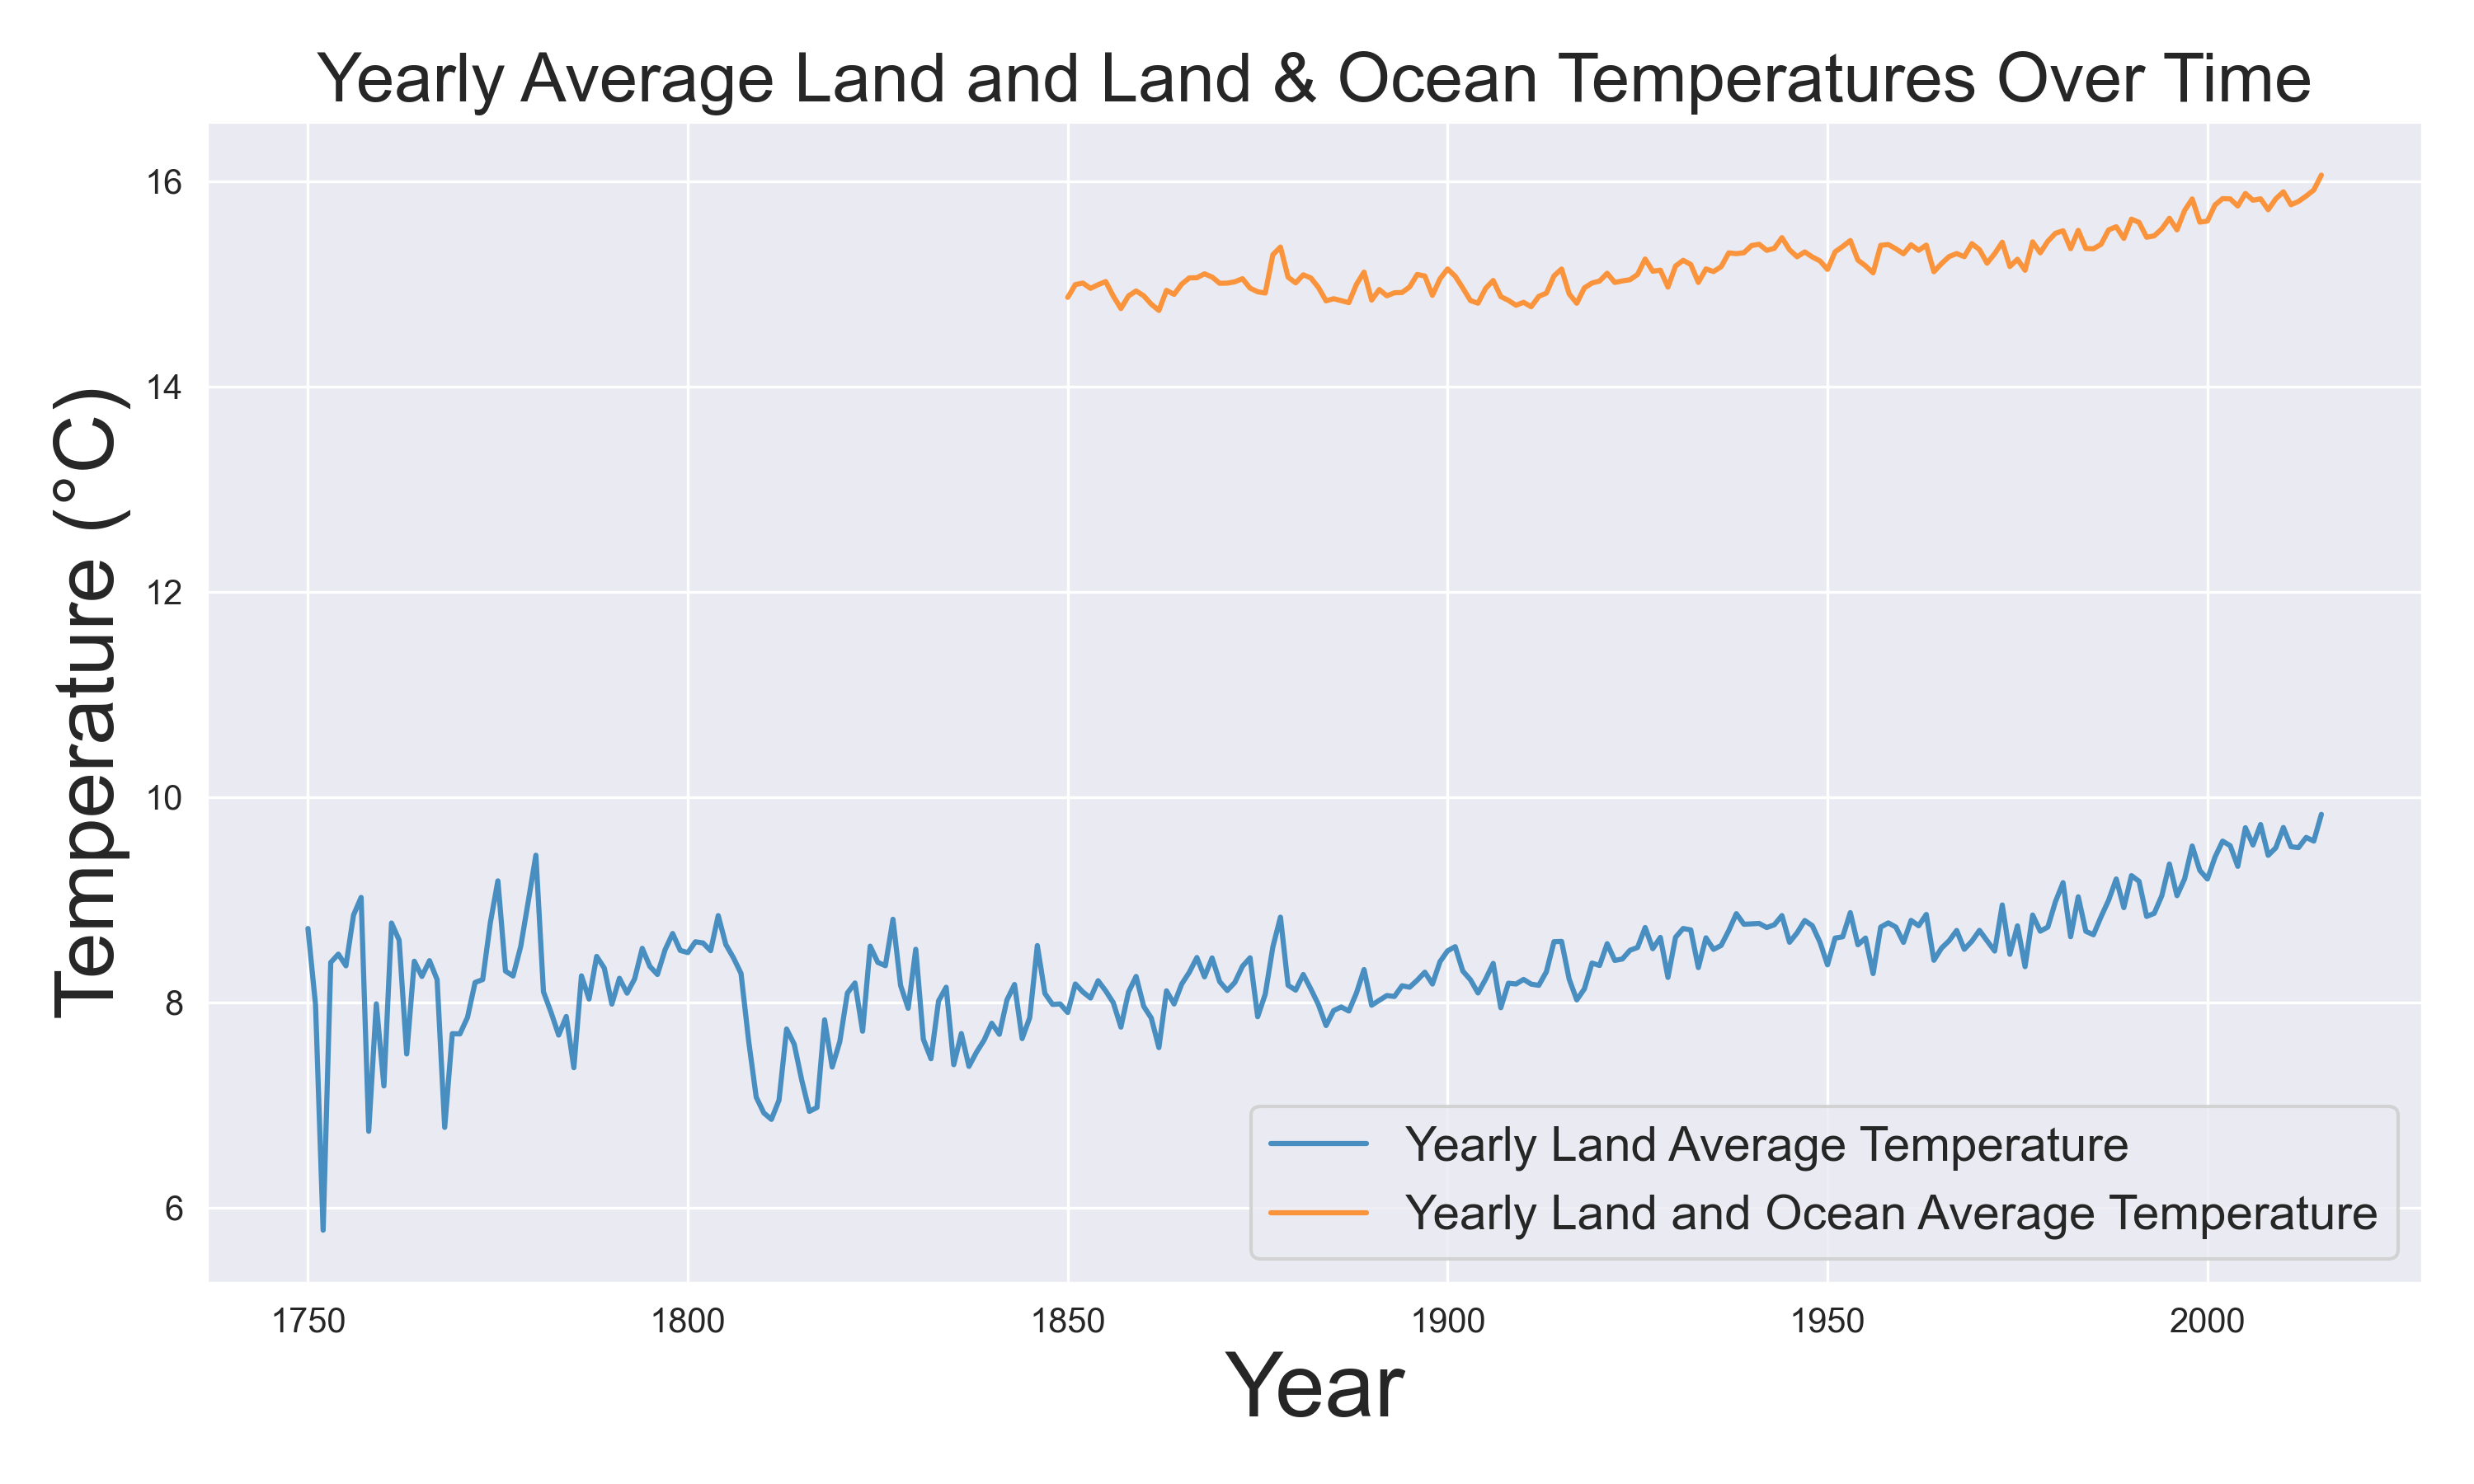
\includegraphics[width=\columnwidth]{CPSC483ClassProjectTemplate/images/Land_and_Ocean_Average_Temperature_Over_Time.png}
\caption{Land and Ocean Average Temperature.}
\label{fig:temperature_plot}
\end{figure}

Although the dataset lacks ocean temperature records from 1750 to 1850, the available data demonstrates a clear trend of rising temperatures in the years that followed, as shown in Figure~\ref{fig:temperature_plot}. Notably, the average uncertainty in the measurements, illustrated in Figure~\ref{fig:temperature_uncertainty_plot}, has steadily decreased over time, reflecting advancements in measurement techniques and modeling methodologies. This improved accuracy strengthens the reliability of the dataset and reinforces the observation that global temperatures have been consistently increasing, even as measurement precision has improved.

\begin{figure}[htbp]
\centering
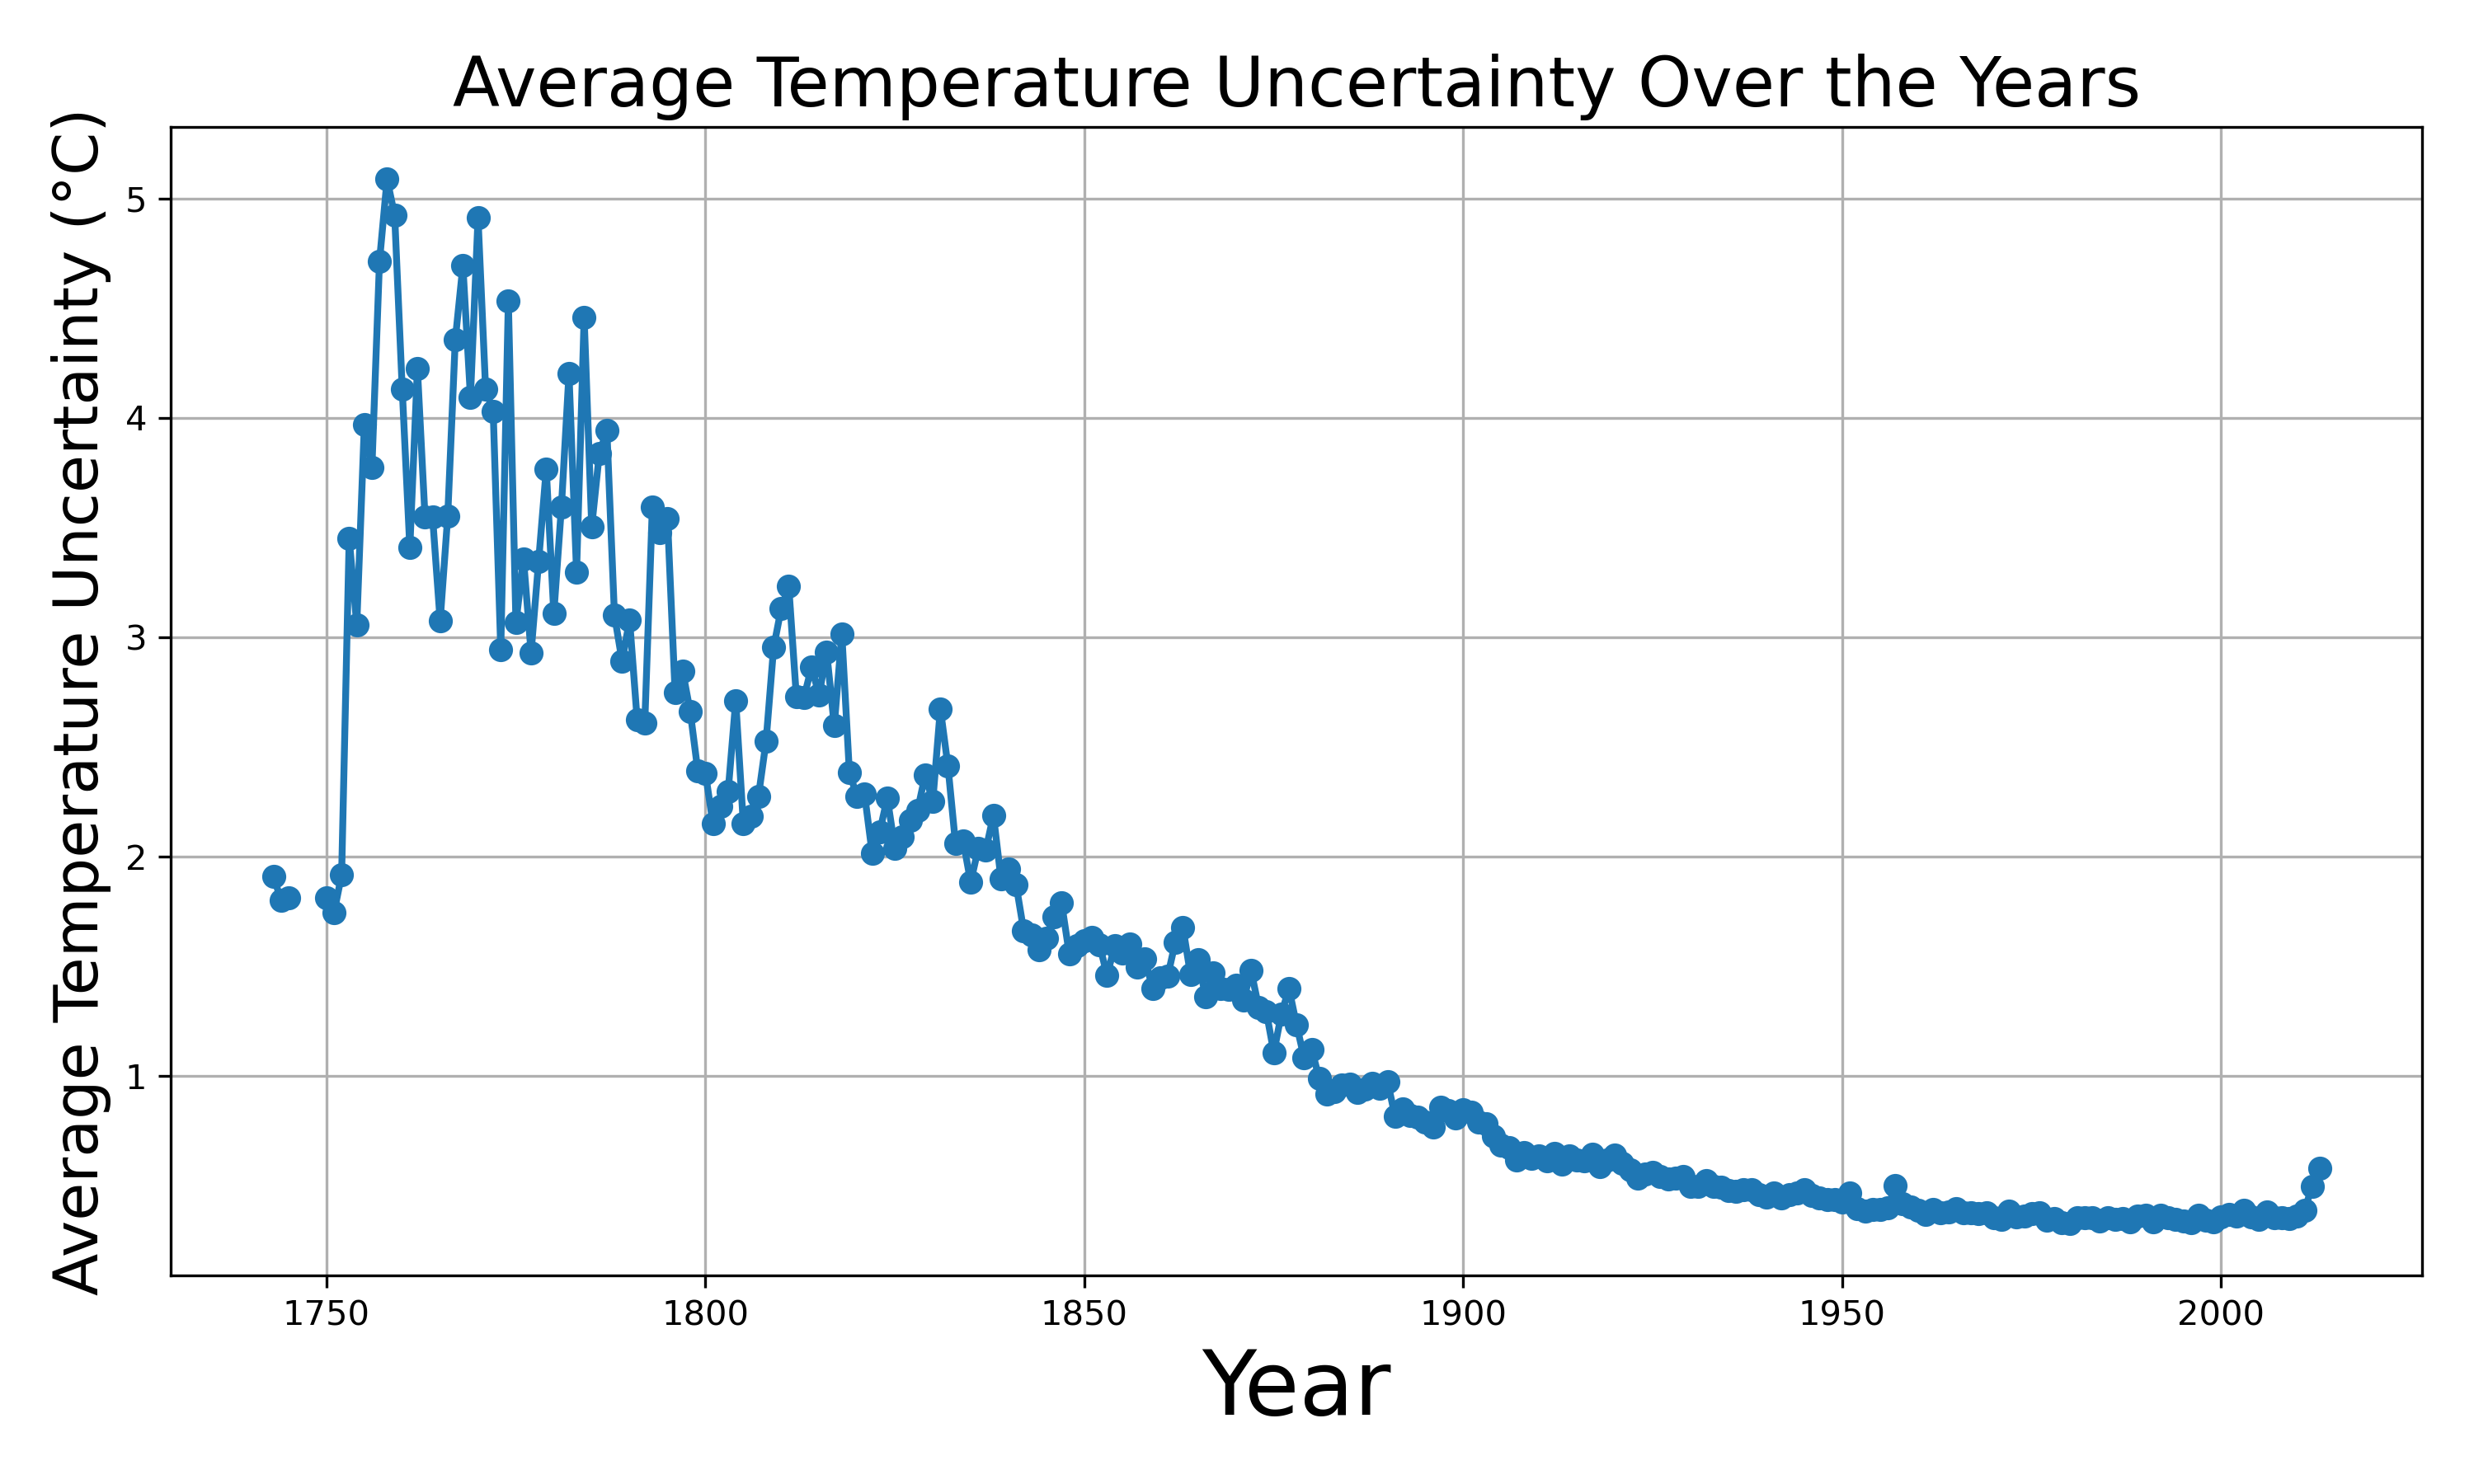
\includegraphics[width=\columnwidth]{CPSC483ClassProjectTemplate/images/Average_Temperature_Uncertainty_Over_Years.png}
\caption{Average Temperature Uncertainty Over the Years}
\label{fig:temperature_uncertainty_plot}
\end{figure}

\section{Methods}

This section explains the approach, including data sourcing and preparation, feature extraction for analysis, and the machine learning techniques applied to build the prediction models.

\subsection{Climate Change Dataset}
The dataset used for this study is obtained from the Berkeley Earth Surface Temperature project, focusing on recorded land temperatures across various cities worldwide. Each record includes the average land temperature (AverageTemperature) and its corresponding uncertainty value (AverageTemperatureUncertainty), which provides the 95\% confidence interval\cite{b6}\cite{b7}. Additional fields in the dataset include the date of the measurement, the city and country where the measurement was recorded, and the location's geographic coordinates (latitude and longitude).

For this analysis, data starting from 1870 is used to ensure consistency, as earlier records were incomplete. Entries with missing values in the AverageTemperature field are removed to maintain the integrity of the dataset. This cleaned subset provides a comprehensive view of global land temperatures over time, enabling a focused analysis of spatial and temporal patterns.

\subsection{Features}

The dataset provides several fields, each evaluated for its potential contribution to improving the predictive power of machine learning models. After thorough analysis, the following features are selected and processed for experimentation:

\subsubsection{Year and Month}
Extracted from the dt (date) field, these temporal components are essential for capturing seasonal and yearly trends. The dt field was decomposed into two distinct numerical features, enabling models to detect periodic patterns in temperature changes. These features were especially important for aligning historical data with future forecasting requirements.

\subsubsection{Latitude and Longitude}
Geographic coordinates are included as key spatial features to account for regional climate variability. These fields were initially represented as strings, such as “4.02N” for latitude and “76.34W” for longitude. To make them usable for machine learning models, the values were converted into numerical representations:

\begin{itemize}
\item \textbf{North (N)} and \textbf{East (E)} coordinates were kept positive.
\item \textbf{South (S)} and \textbf{West (W)} coordinates were converted to negative values.
\end{itemize}

This transformation ensured that the data accurately reflected global positioning and could be directly utilized in spatial modeling.
The conversion process ensured consistency across the dataset, enabling the models to interpret latitude and longitude as meaningful numerical features.

\subsubsection{Country and City}
These are explored as categorical features using one-hot encoding to differentiate regions beyond latitude and longitude. However, these features did not contribute significantly to model performance, possibly due to its redundancy with spatial coordinates. They were excluded from the final experiments to reduce model complexity.

\subsubsection{AverageTemperatureUncertainty}
Initially included as a feature, this variable measures the 95\% confidence interval of the temperature readings. While it shows a high correlation with the target variable, it is excluded from the experiments. In a real-world scenario, this uncertainty measure is not available for future predictions, and its inclusion leads to overfitting by providing information that unrealistically benefits the model.

The AverageTemperature variable represents the land surface temperature in degrees Celsius and serves as the target variable predicted by all models in this work. This value directly measures climatic conditions and offers valuable insights into global warming trends. By predicting this variable, the model’s performance can be evaluated effectively, highlighting its ability to accurately uncover patterns in historical climate data and predict future conditions.

After iterative testing and refinement, the final set of features consists of Year, Month, Latitude, and Longitude. This selection is made for its simplicity and real-world applicability, offering a balanced representation of both temporal and spatial dimensions. These features ensure that the model’s predictions are interpretable and practical for forecasting.

By focusing on these features, this work ensures the development of robust and generalizable models, avoiding pitfalls associated with overfitting or information leakage.

\subsection{Machine Learning Classifiers}
We chose four different machine-learning algorithms to train and test the data we selected: Linear Regression, Random Forest, K-Nearest Neighbor, and Support Vector Machine.  

\subsubsection{Linear Regression}
Due to the pattern of growth our group recognized in our selected data, we chose to start with a linear regression model. In addition, linear regression provides a strong baseline to compare with other prediction models. Linear regression also provides an effective visual model for viewing, as shown in Figure~\ref{fig:linear_regression_plot}, which illustrates the actual versus predicted temperatures. . This model is also very computationally efficient, allowing for much more testing and updating.

\begin{figure}[htbp]
\centering
\includegraphics[width=\columnwidth]{CPSC483ClassProjectTemplate/images/Actual_vs_Predicted_LinearSVR_M1.png}
\caption{Actual vs. Predicted Temperatures for Linear Regression Model.}
\label{fig:linear_regression_plot}
\end{figure}

The linear regression model's \(R^2\) score is 0.1391. Even though the model shows a considerably weak relationship, it provides key visualizations and guidance for improving the performance of other models.

\subsubsection{Random Forest}
The Random Forest Regressor was selected for its capability to handle non-linear relationships and its robustness against over-fitting due to the ensemble nature of the algorithm, as well as its feature importance and flexibility. 

Random forest is selected because it better captures non-linear relationships. Insights from the linear regression model guide the shift to non-linear models. As shown in the results, non-linear models prove to be significantly more accurate.

This type of model is also very robust to overfitting. Using an average of all the predictions across multiple trees provides a much more generalized prediction. This can be further tuned with hyperparameters. 

Feature importance is an essential aspect that random forest provides, as none of the other models perform comparatively well in this regard. Random forest offers insights into which features are the most influential when the model makes its predictions.

Flexibility is another reason why this model is selected. Since random forest uses a series of decision trees to make predictions, the model can effectively utilize continuous and categorical features.

\begin{figure}[htbp]
\centering
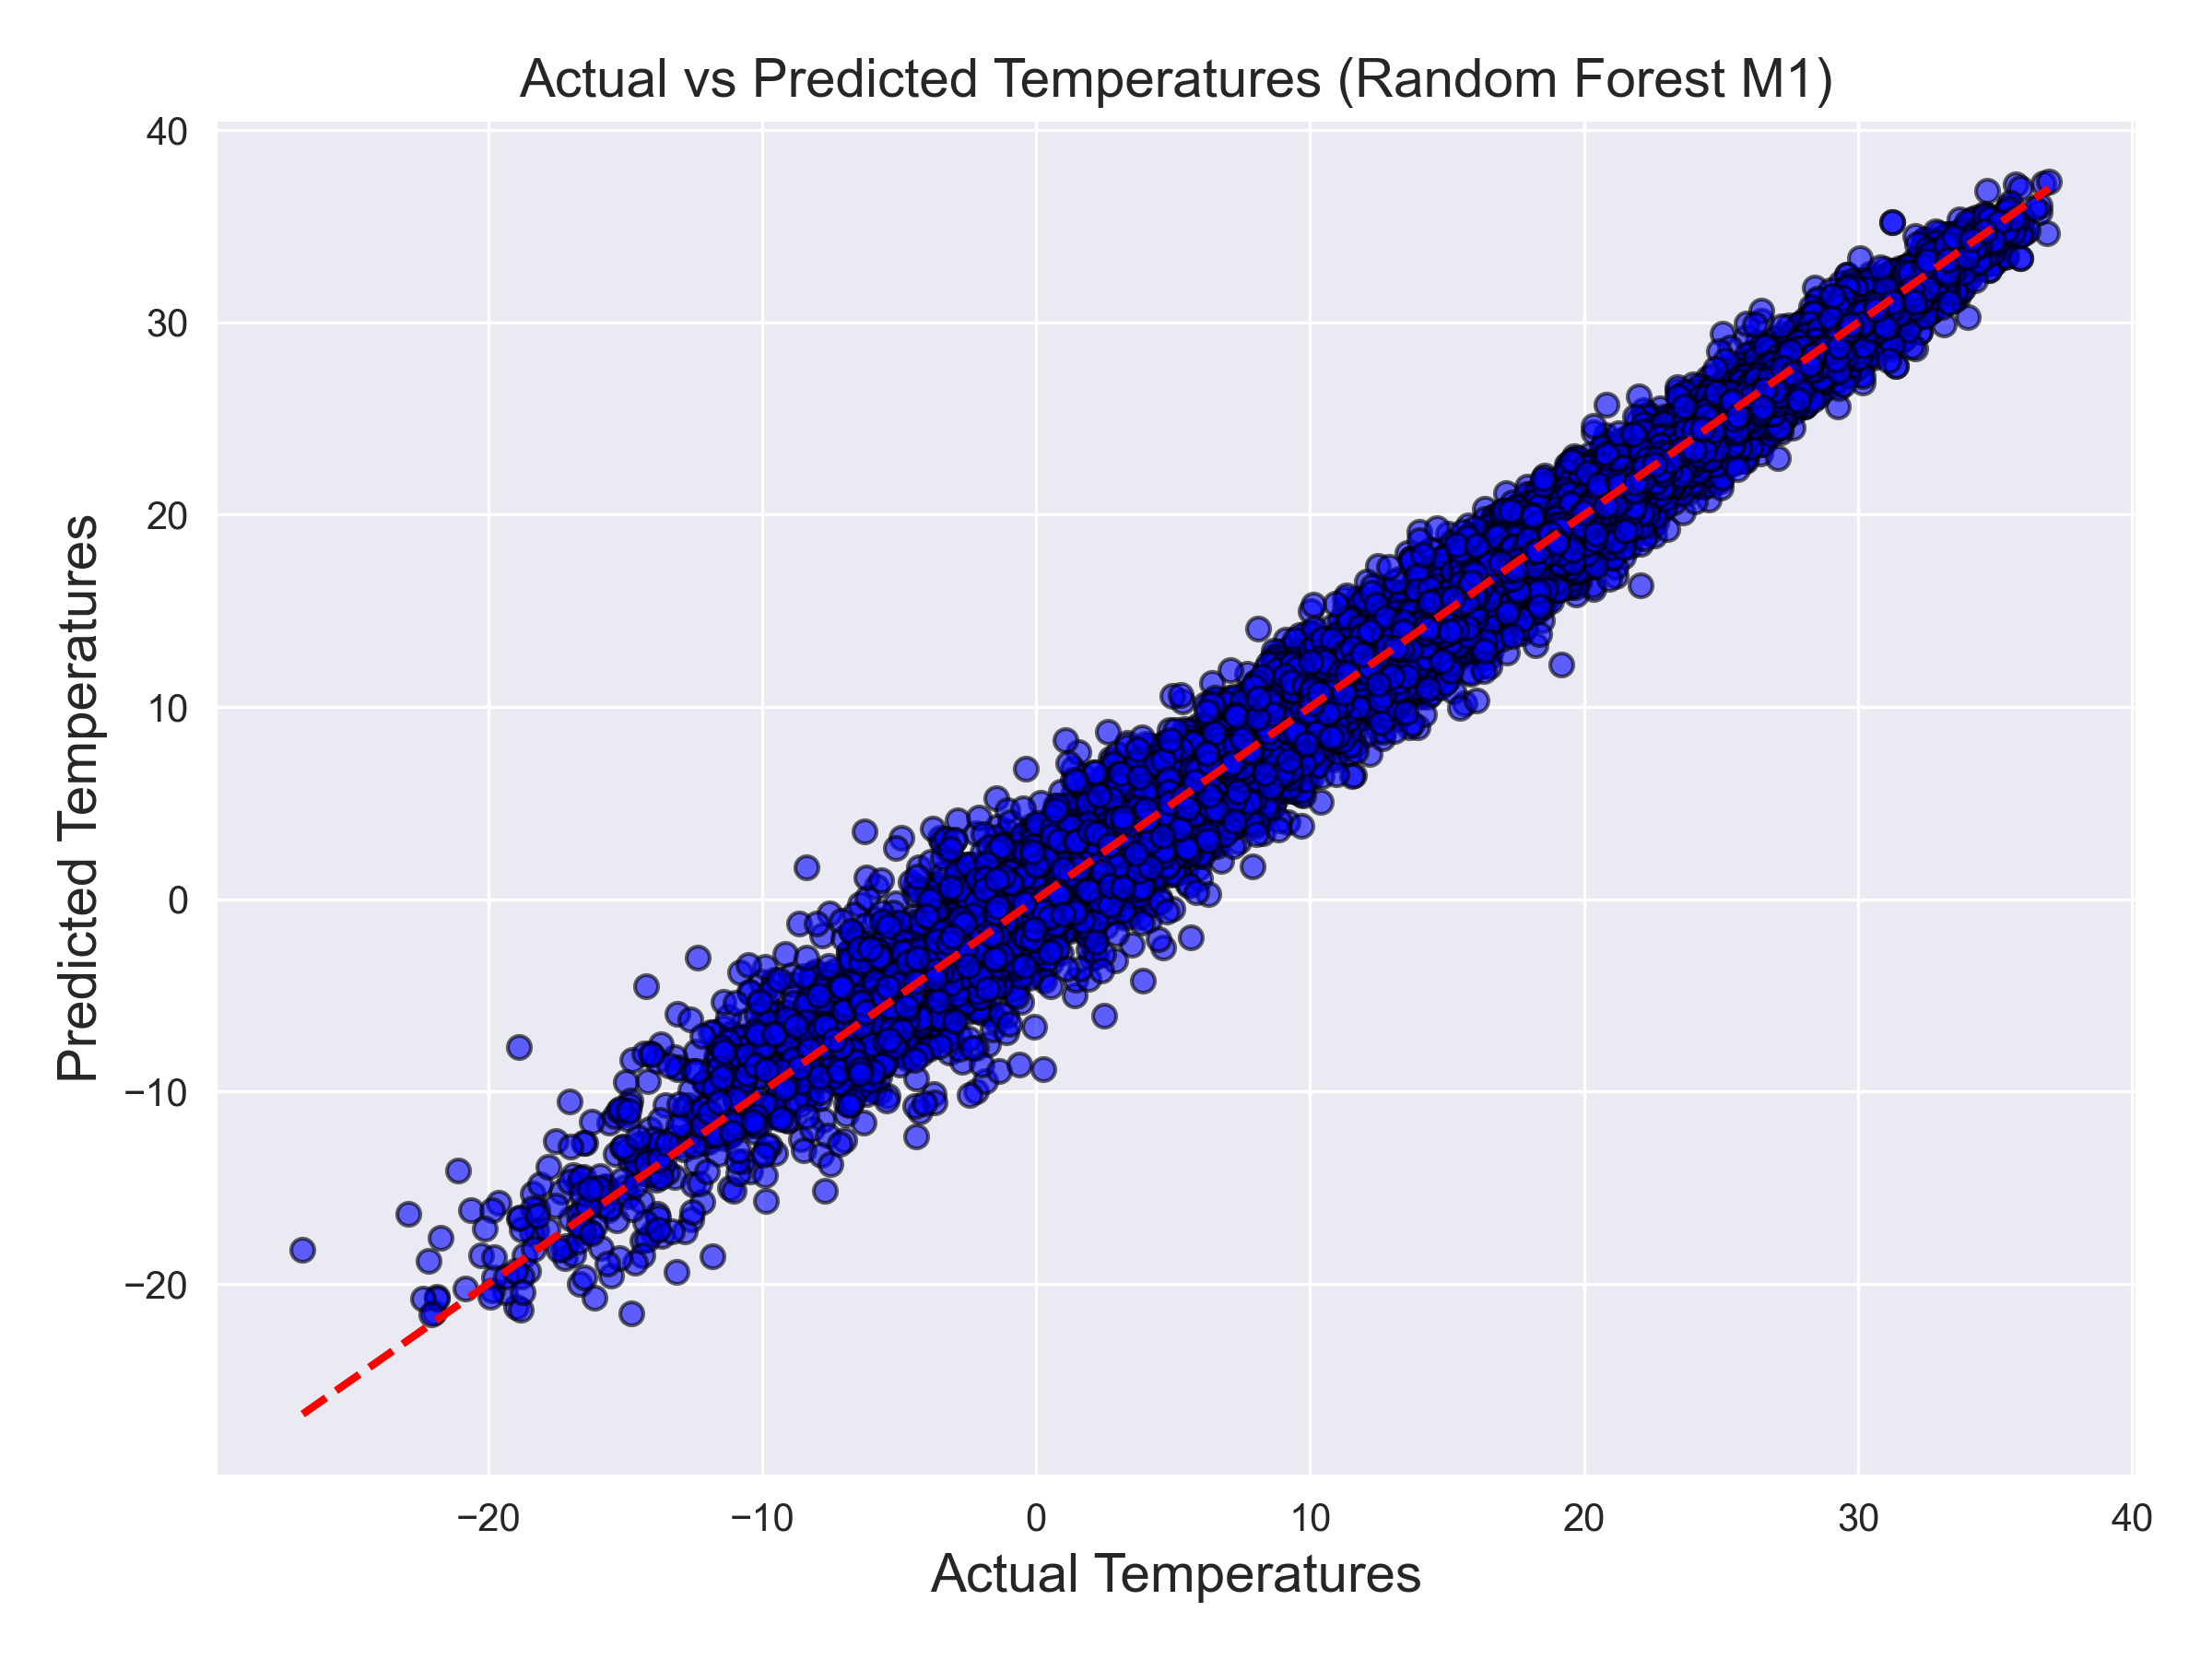
\includegraphics[width=\columnwidth]{CPSC483ClassProjectTemplate/images/Actual_vs_Predicted_Random_Forest_M1.png}
\caption{Actual vs. Predicted Temperatures for Random Regression Model.}
\label{fig:random_forest_plot}
\end{figure}

In terms of performance, the Random Forest model produced an exceptional \(R^2\) score of 0.9857, demonstrating its ability to explain 98.57\% of the variance in the test data. As shown in Figure~\ref{fig:random_forest_plot}, the model's predictions closely align with the actual temperature values, highlighting its strong predictive capability.

\subsubsection{Support Vector Regression}
Support Vector Regression (SVR) is selected for its ability to model non-linear relationships, robustness to outliers, and strong generalization across complex datasets.

Building on the results of the linear regression model, which tested for linear relationships, we opted for SVR to explore non-linear patterns in the data. This decision is informed by the observed limitations of linear regression in capturing the complexity of climate data. SVR allows for a more flexible approach by incorporating kernel functions to better model non-linearity.

The resistance to outliers is particularly valuable when analyzing weather data, which often includes anomalies such as irregular weather patterns, solar events, or other unexpected fluctuations. This robustness enhances the model's predictive accuracy by minimizing the impact of these anomalies.

Generalization is another important aspect of the selection of this model. By balancing model complexity with accuracy, SVR reduces the risk of overfitting, ensuring reliable performance even with large datasets. This is crucial for maintaining computational efficiency while achieving accurate predictions.

To further optimize the Support Vector Regression (SVR) model, multiple kernels were tested, including linear, polynomial (poly), and radial basis function (RBF). Each kernel was evaluated based on its ability to model the data accurately while maintaining computational efficiency. Among these, the RBF kernel emerged as the most effective, achieving the highest predictive performance with an \(R^2\) score of 0.9179. As shown in Figure~\ref{fig:SVR_plot_1}, the RBF kernel demonstrates a strong alignment between the actual and predicted values, capturing the non-linear relationships inherent in the dataset and making it the most suitable choice for this application.

\begin{figure}[htbp]
\centering
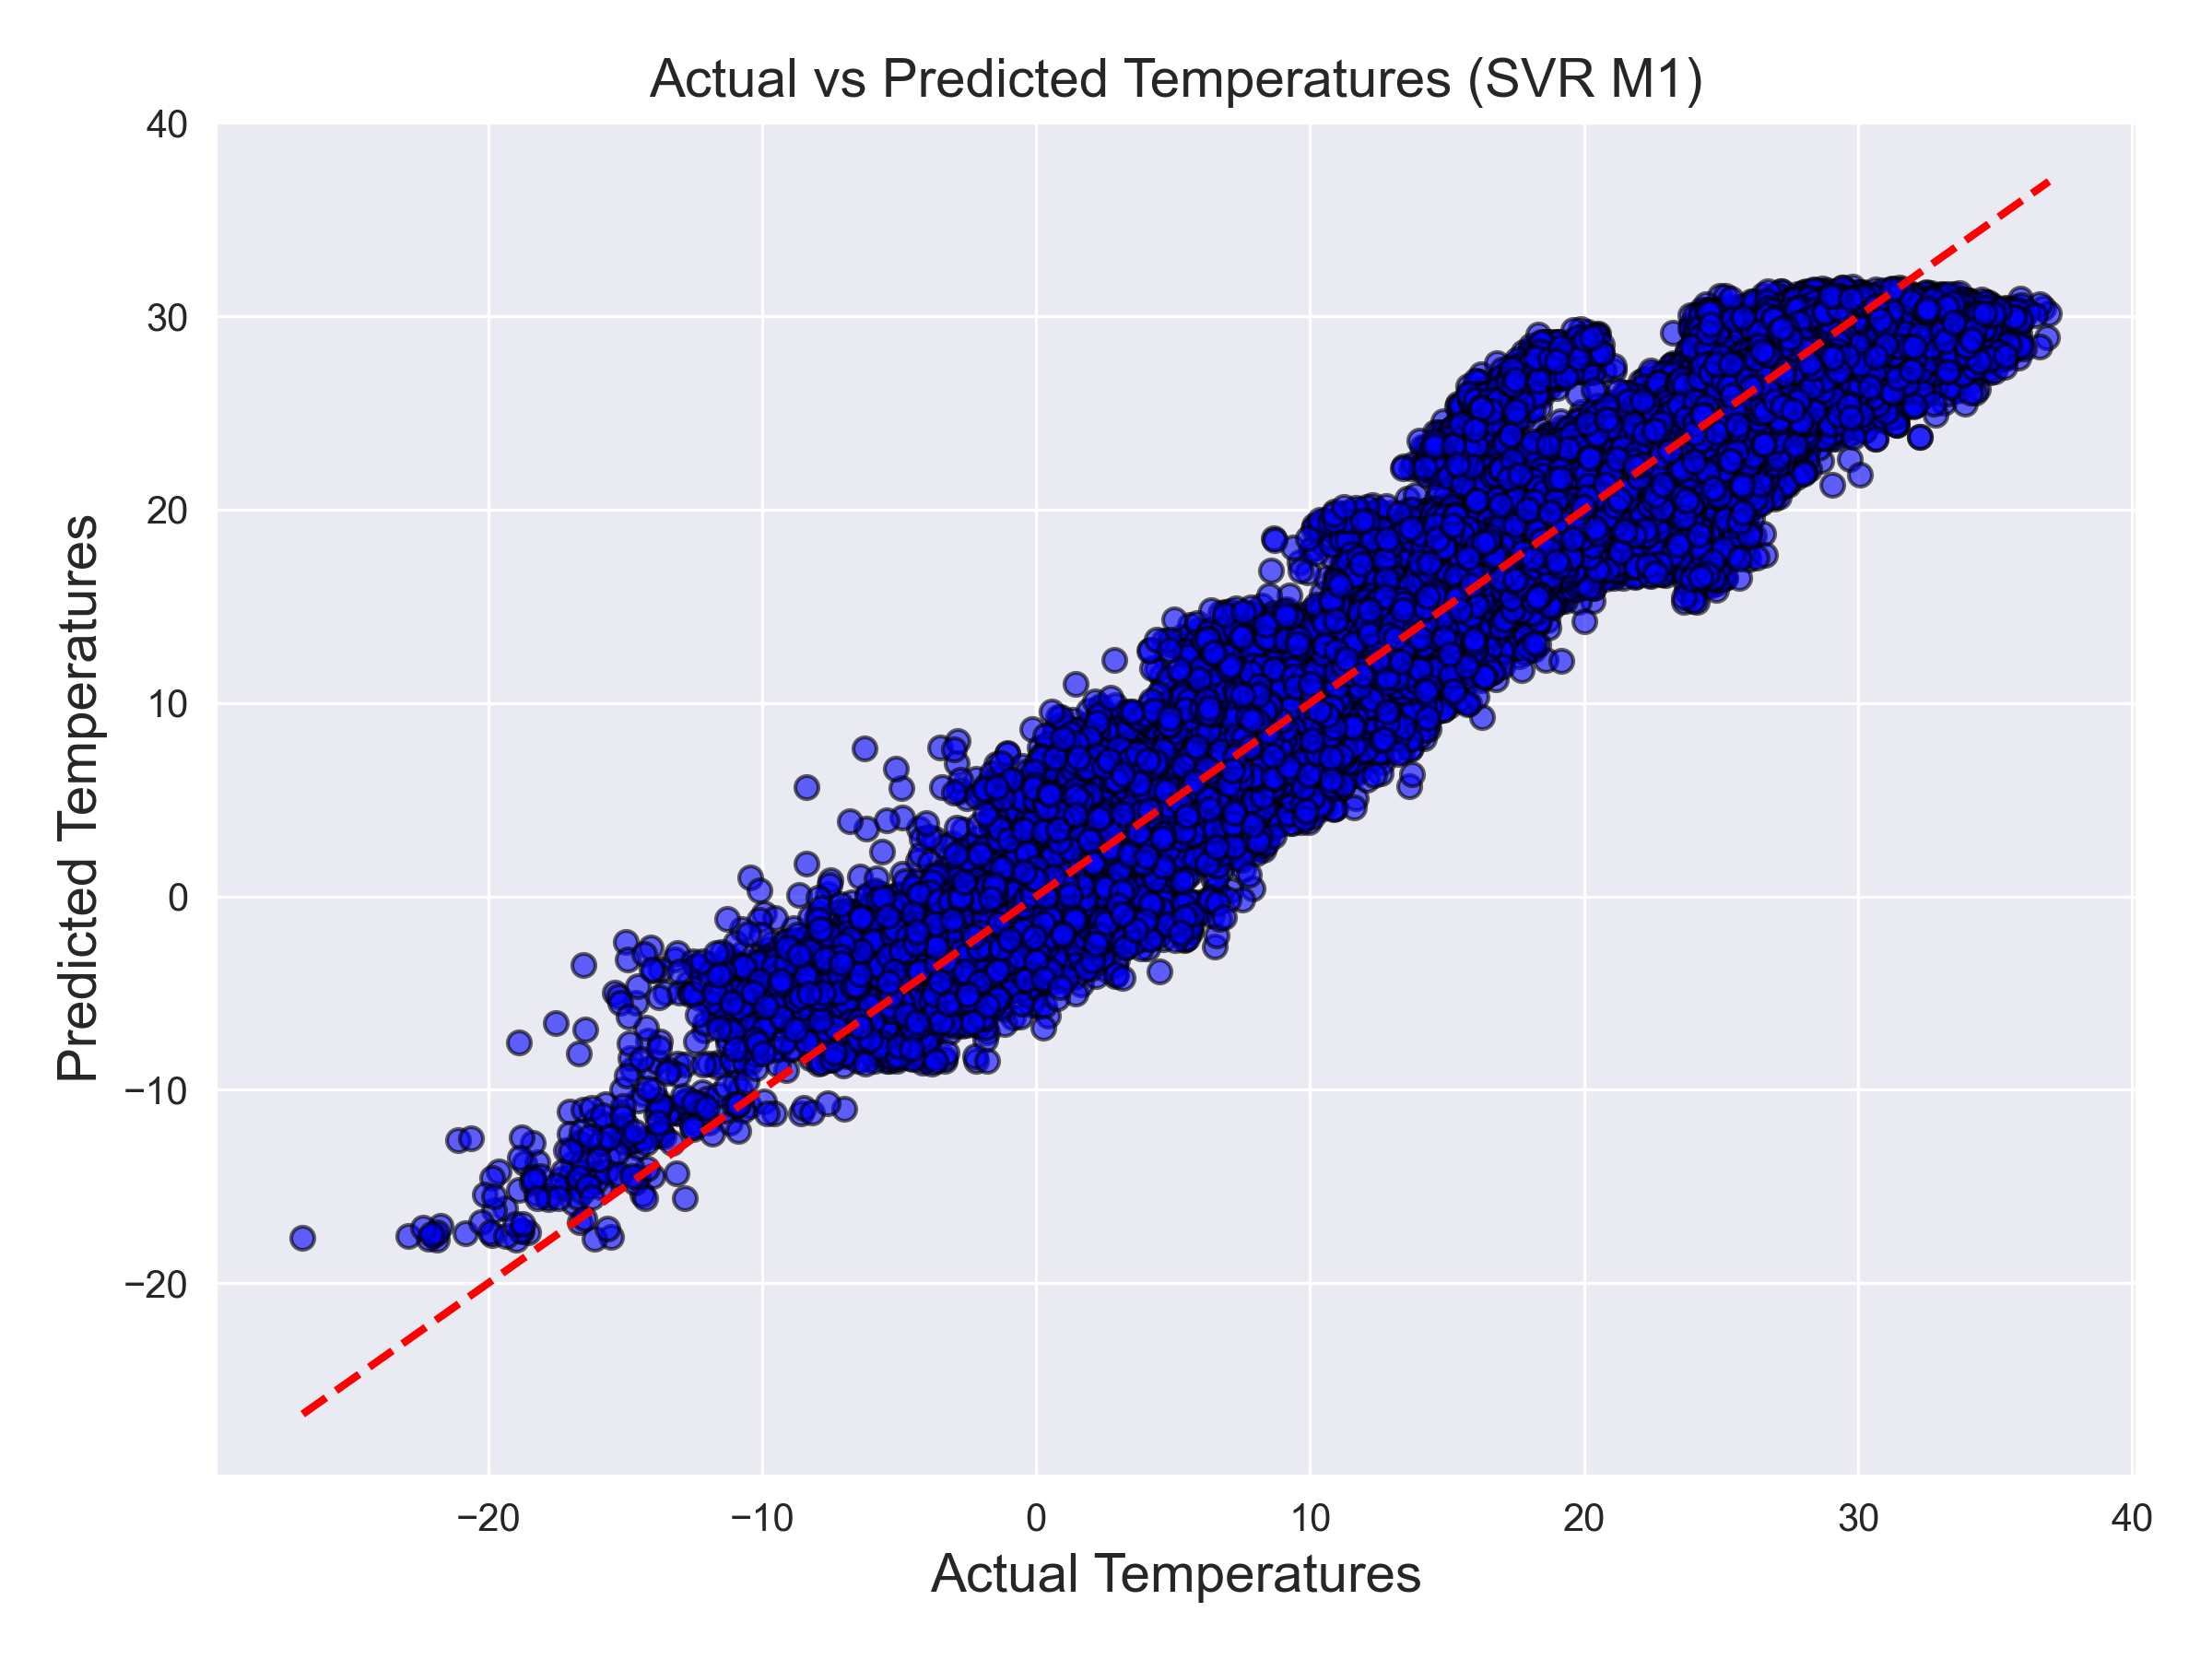
\includegraphics[width=\columnwidth]{CPSC483ClassProjectTemplate/images/Actual_vs_Predicted_SVR_M1.png}
\caption{Actual vs. Predicted Temperatures for SVR with 'RBF' Kernel.}
\label{fig:SVR_plot_1}
\end{figure}
The SVR model with the RBF kernel significantly outperforms both the linear and polynomial kernels. The linear kernel, as illustrated in Figure~\ref{fig:SVR_plot_3}, struggles to align the predicted values with the actual data, achieving an \(R^2\) score of just 0.0835. This poor performance highlights its inability to model the complexity of the dataset. The polynomial kernel, while better than the linear kernel, achieves only moderate alignment, as seen in Figure~\ref{fig:SVR_plot_2}, and produces an \(R^2\) score of 0.3741. This demonstrates the limitations of the polynomial kernel in effectively capturing the intricacies of the dataset compared to the RBF kernel.

\begin{figure}[htbp]
\centering
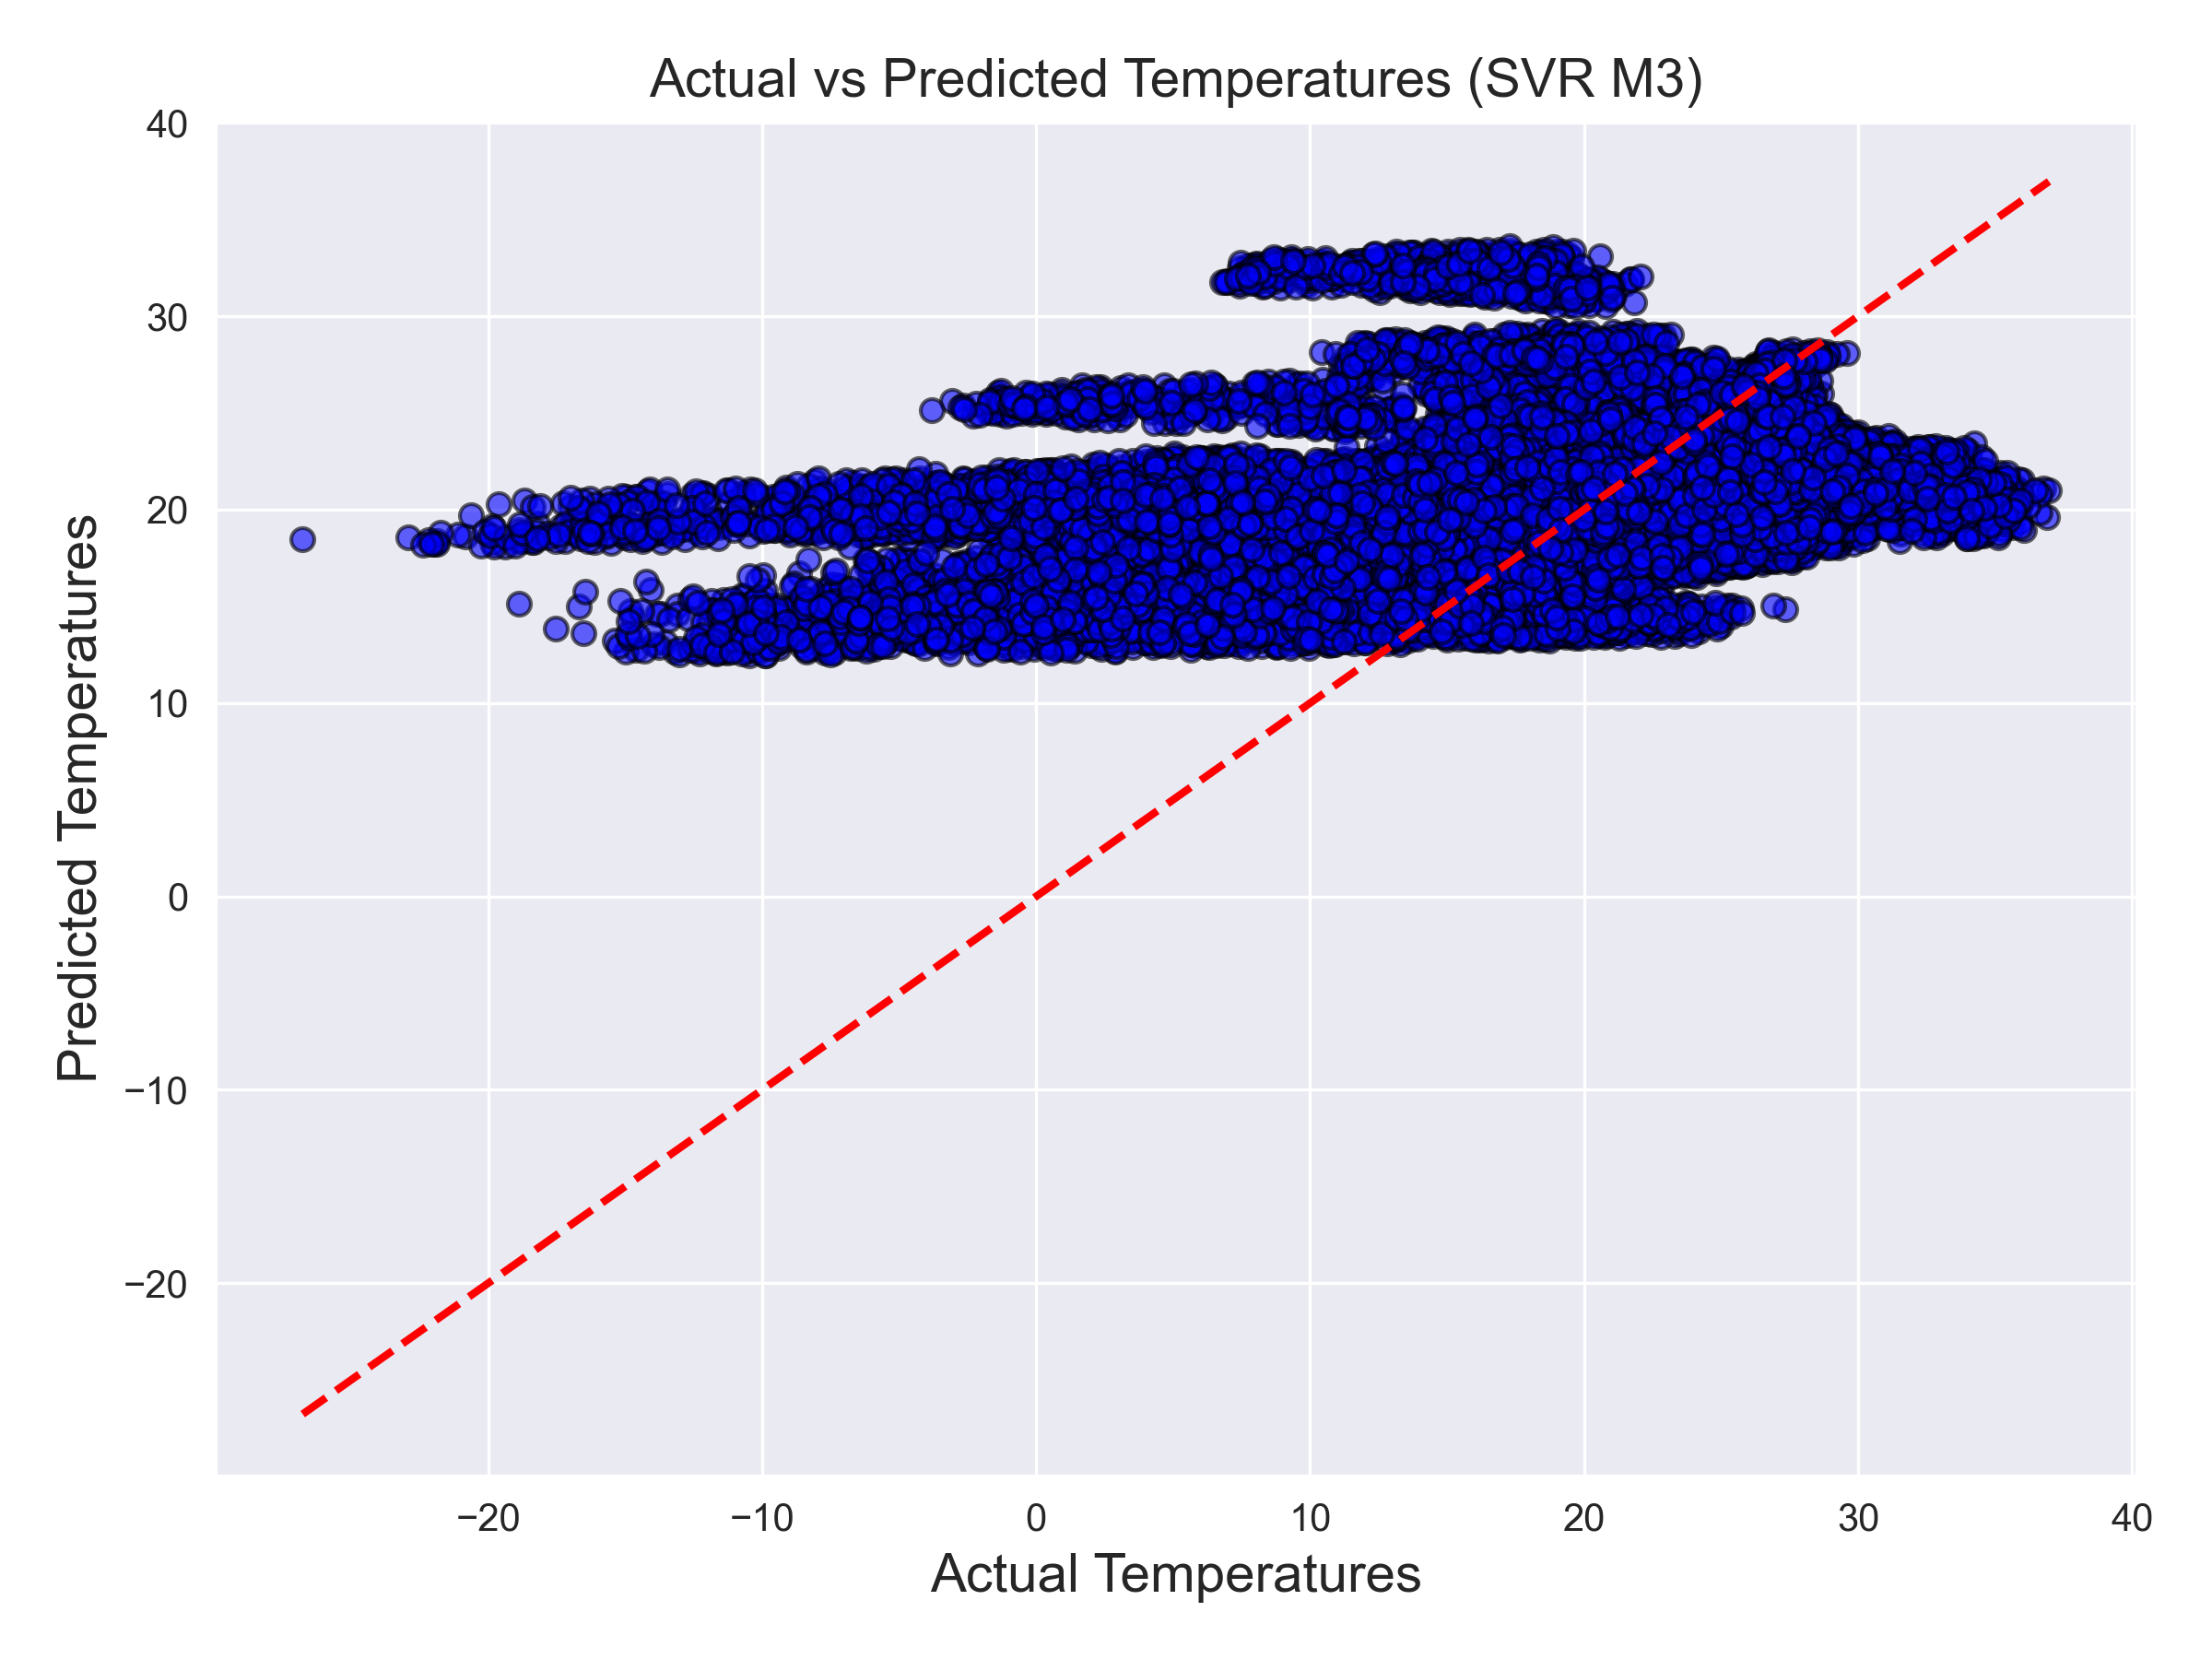
\includegraphics[width=\columnwidth]{CPSC483ClassProjectTemplate/images/Actual_vs_Predicted_SVR_M3.png}
\caption{Actual vs. Predicted Temperatures for SVR with 'Linear' Kernel.}
\label{fig:SVR_plot_3}
\end{figure}

\begin{figure}[htbp]
\centering
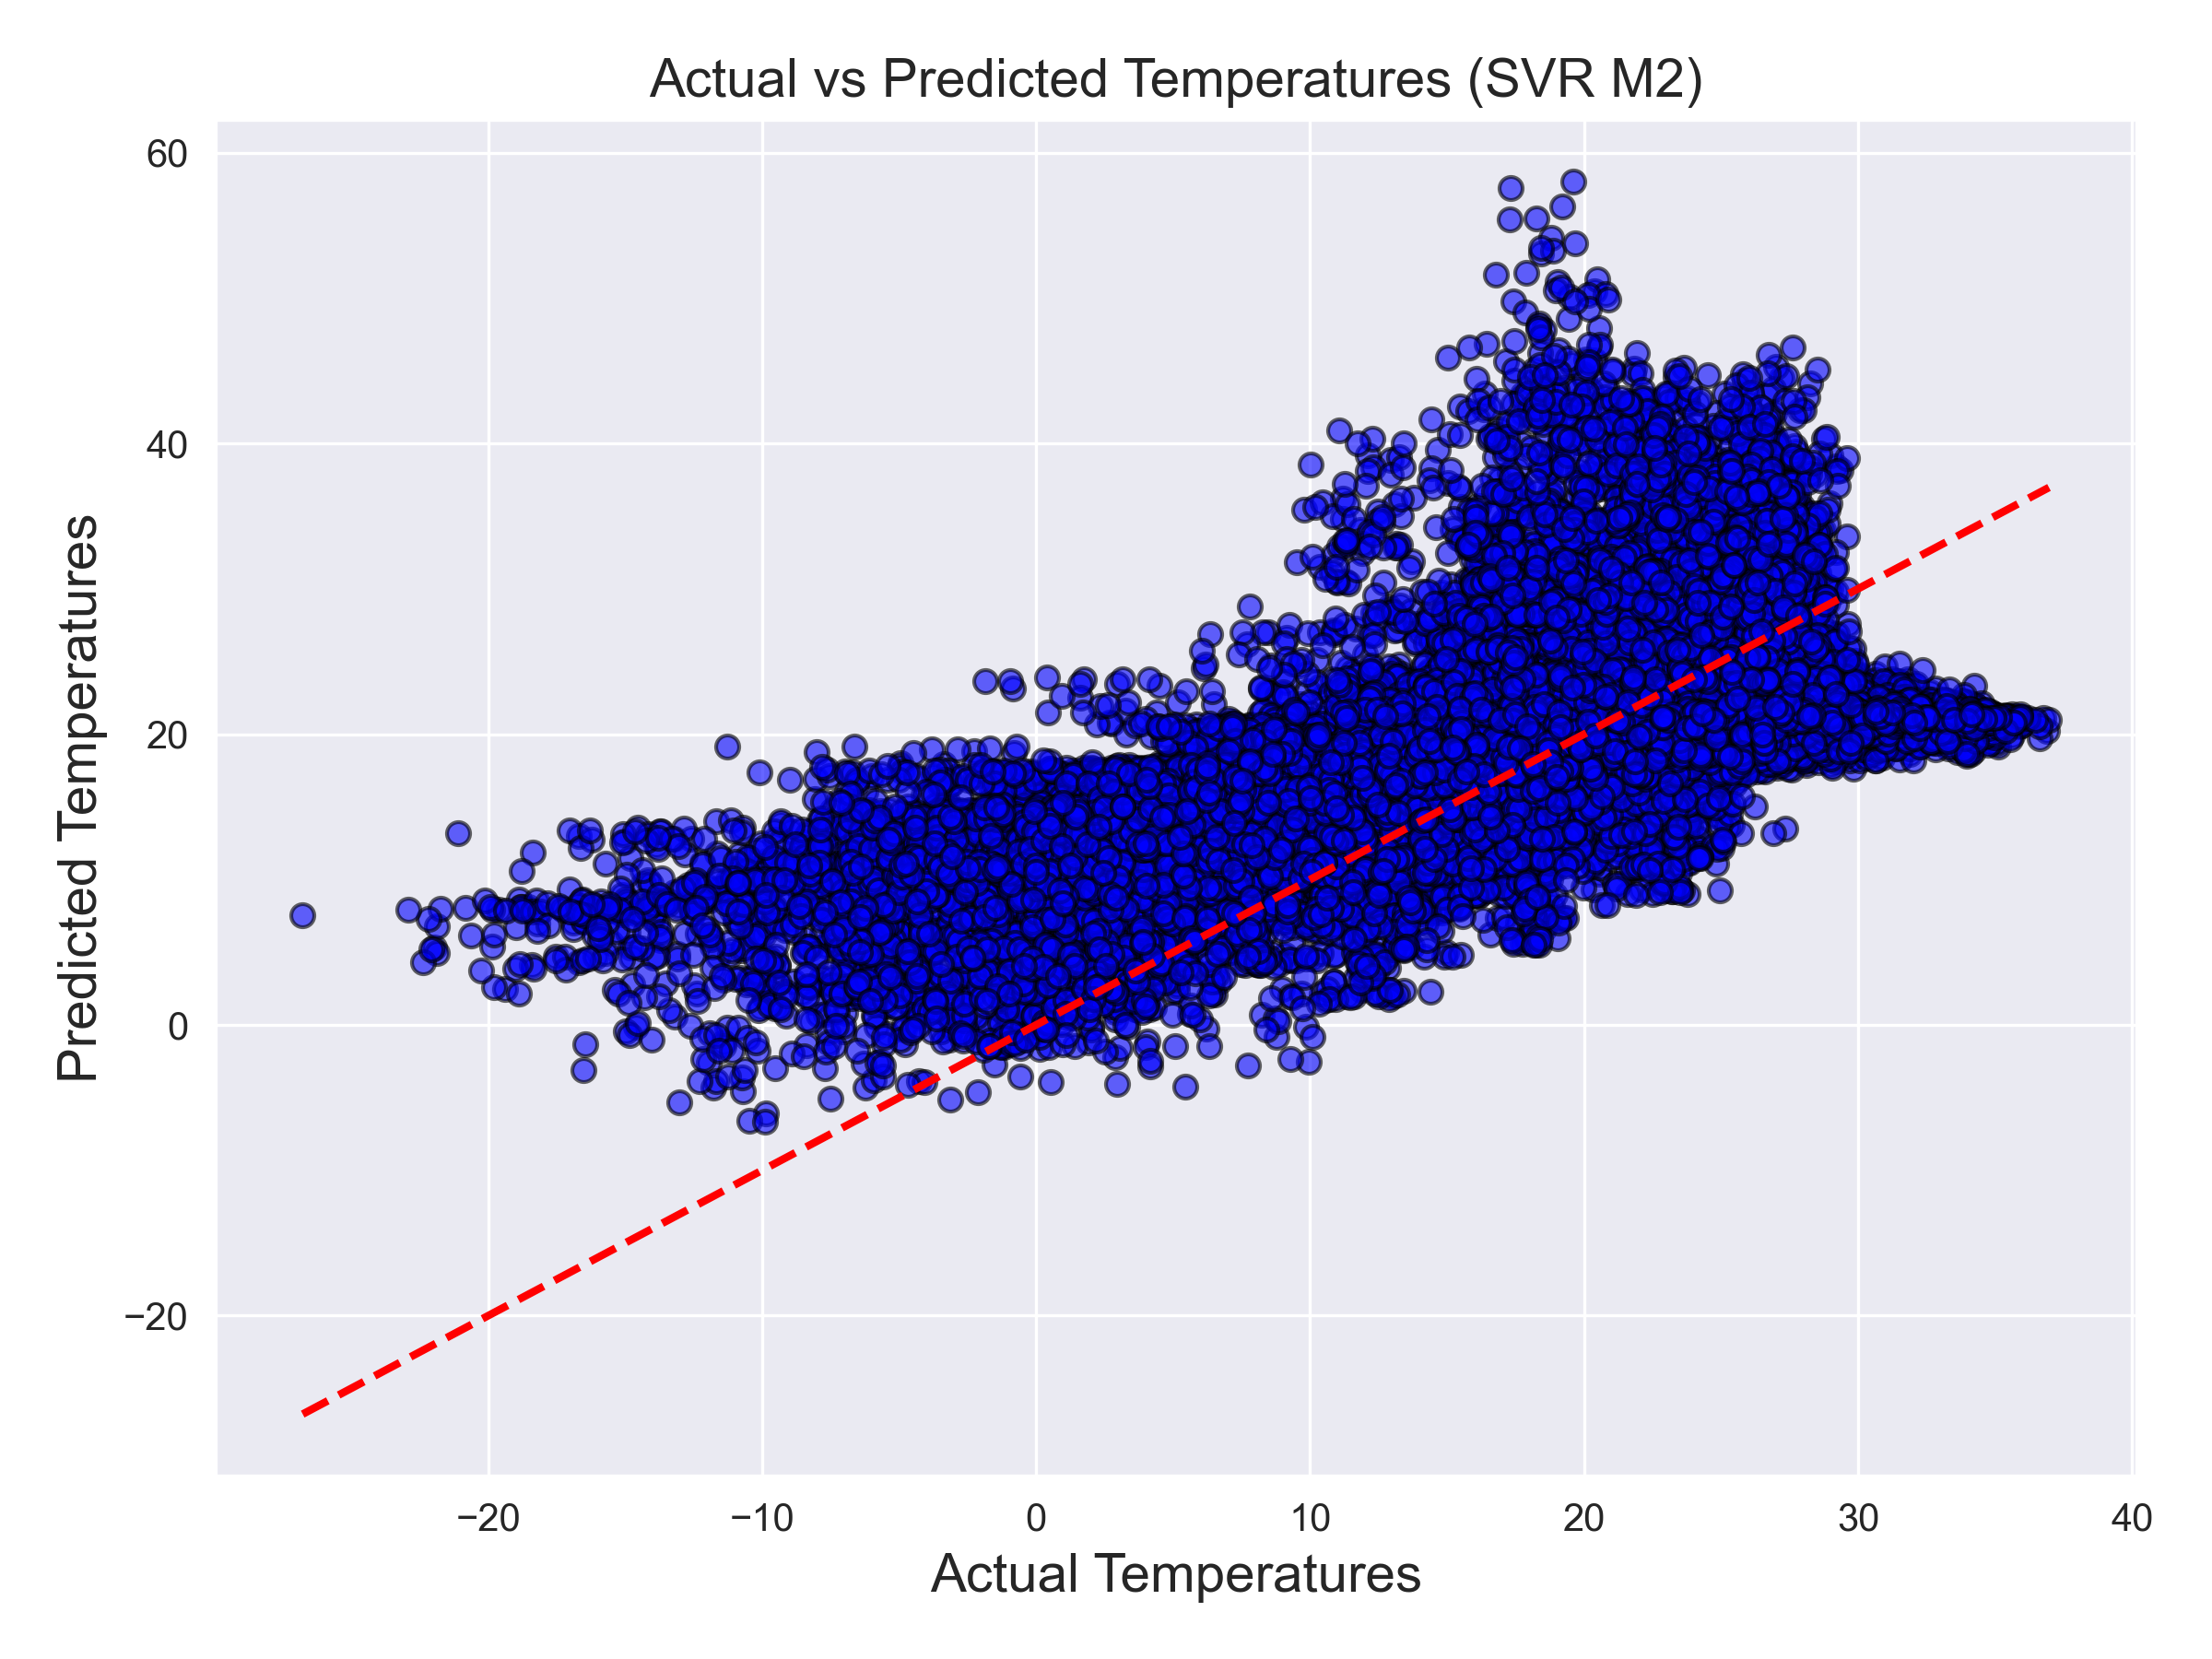
\includegraphics[width=\columnwidth]{CPSC483ClassProjectTemplate/images/Actual_vs_Predicted_SVR_M2.png}
\caption{Actual vs. Predicted Temperatures for SVR with 'Poly' Kernel.}
\label{fig:SVR_plot_2}
\end{figure}

This comparison underscores the value of non-linear kernel functions in achieving accurate predictions for datasets with intricate relationships between features and target values.


\subsubsection{K-Nearest Neighbor}
The K-Nearest Neighbor (KNN) regressor is selected for its simplicity and effectiveness in capturing local patterns in the dataset. The KNN algorithm operates by averaging the target values of the \(k\)-nearest data points in feature space, making it highly effective for non-linear datasets with complex spatial and temporal relationships. The optimal value of \(k\) was determined through hyperparameter tuning, with \(k = 5\) yielding the best results in terms of predictive accuracy.

The KNN model achieves an \(R^2\) score of 0.9706, falling slightly behind Random Forest but still demonstrating strong performance. Figure~\ref{fig:KNN_plot} illustrates the alignment between actual and predicted values, showcasing the model's effectiveness in capturing spatial and temporal patterns, which are critical for climate data analysis.

\begin{figure}[htbp]
\centering
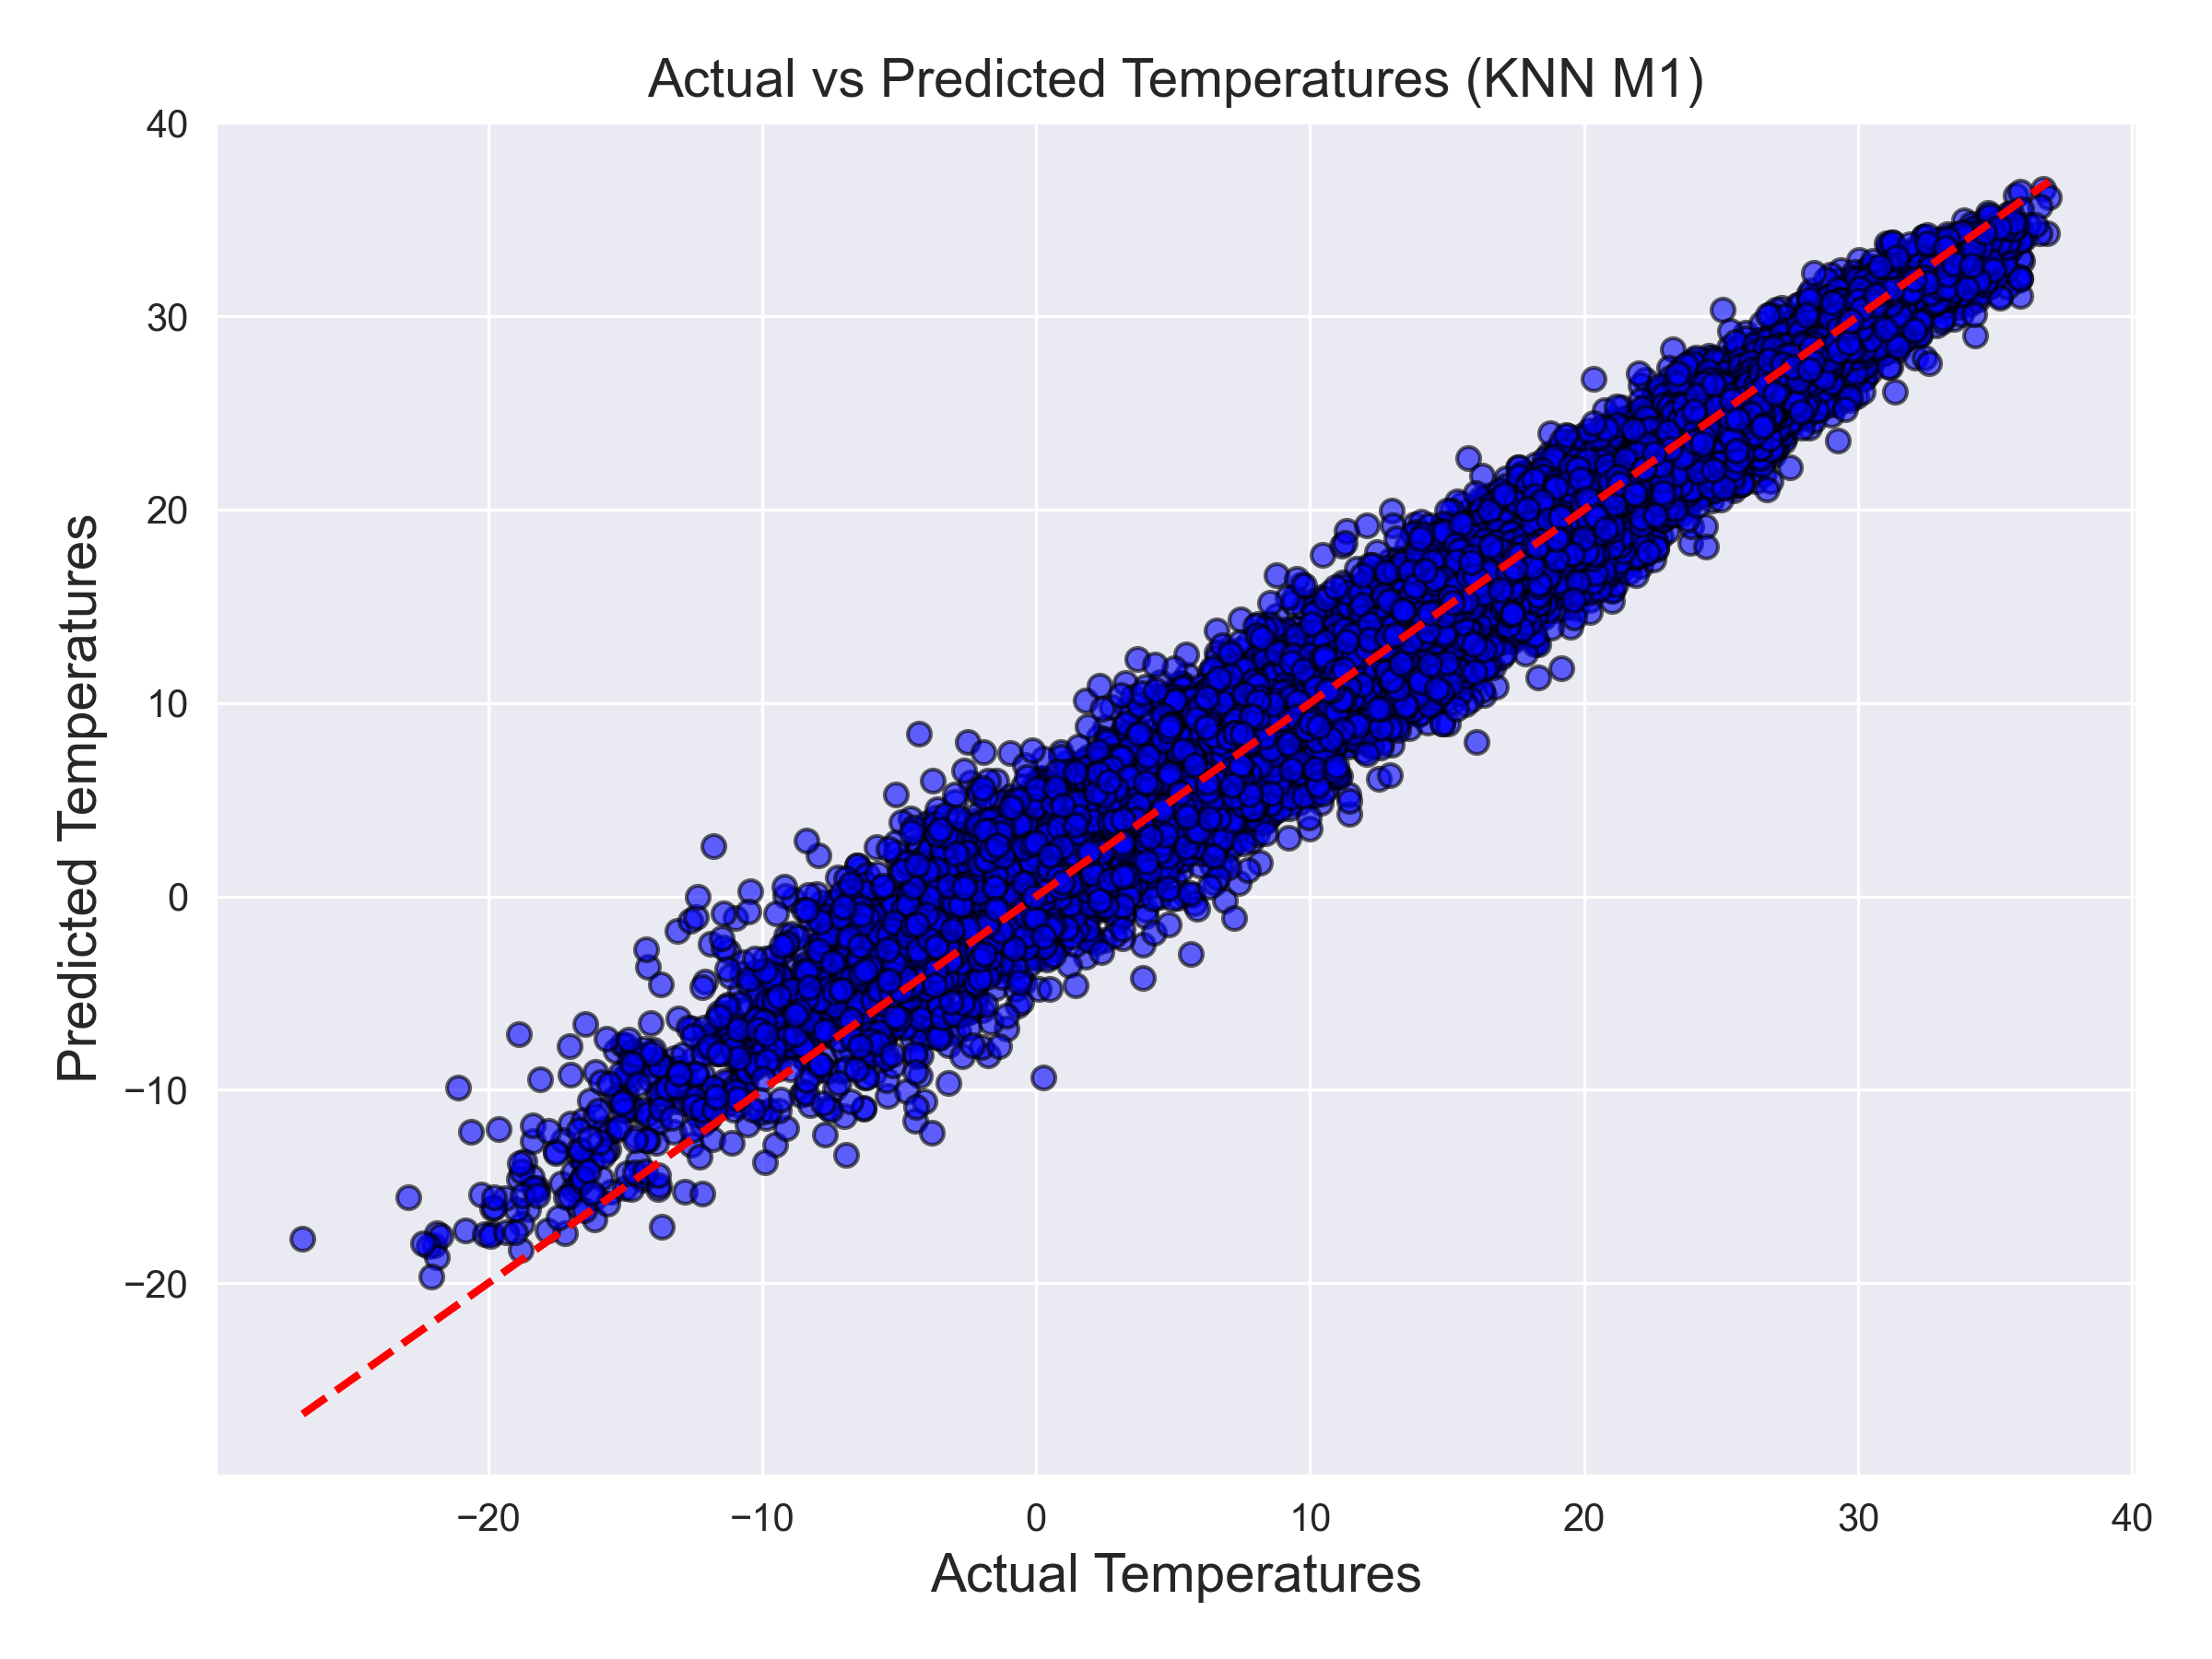
\includegraphics[width=\columnwidth]{CPSC483ClassProjectTemplate/images/Actual_vs_Predicted_KNN_M1.png}
\caption{Actual vs. Predicted Temperatures for KNN.}
\label{fig:KNN_plot}
\end{figure}

\section{Experiments}
This section outlines the experimental setup and analyzes the results of applying machine learning models to the climate dataset. The goal is to compare the performance of multiple models and evaluate their ability to capture spatial and temporal trends in temperature data.
\subsection{Experimental Procedure}
We conducted our experiments by splitting the dataset randomly into an 80\% training set and a 20\% test set. Random splits ensure that the training and testing subsets represent the overall dataset and minimize biases that could arise from systematic patterns in the data and ensure that the models generalize well to unseen data.

Our experiments proceeded as follows:
\begin{enumerate}
    \item \textbf{Select learner:} Linear Regression, Random Forest, Support Vector Regression (SVR), K-Nearest Neighbor (KNN);
    \item \textbf{Select features:} Final features (Year, Month, Latitude, Longitude), reduced features, or additional encoded features (Country);
    \item \textbf{Select model-specific configurations:}
    \begin{itemize}
        \item For SVR, test kernels (Linear, Polynomial, RBF);
        \item For KNN, vary the feature set and evaluate \(k = 5\);
        \item For Random Forest, compare feature sets with and without Country encoding.
    \end{itemize}
\end{enumerate}

Each model was trained on the training set using its respective configuration. The models were then evaluated on the test set, and their performance was measured using \(R^2\) scores. We recorded results for each configuration and compared them to determine the most effective combination of features and model-specific parameters.

\subsection{Model Performance Comparison}
The performance of the models is summarized in Table \ref{tab:model_performance}, which provides their respective \(R^2\) scores on the test set. The results highlight the strengths and limitations of each model.

% create table here
\begin{table}[htbp]
\centering
\caption{Model Performance Comparison}
\label{tab:model_performance}
\begin{tabular}{|l|c|c|}
\hline
Model & Configuration & \(R^2\) Score \\ \hline
Random Forest & Final Features & 0.985694 \\ \hline
Random Forest & With Country Encoding & 0.985666 \\ \hline
KNN & Final Features & 0.970539 \\ \hline
KNN & Reduced Features & 0.428712 \\ \hline
SVR & RBF Kernel & 0.917900 \\ \hline
SVR & Polynomial Kernel & 0.374138 \\ \hline
SVR & Linear Kernel & 0.083536 \\ \hline
Linear Regression & Final Features & 0.139092 \\ \hline
Linear Regression & Reduced Features & 0.129212 \\ \hline
\end{tabular}
\end{table}

% probably need to expand here
% perhaps add graphs of different measures and reference it

\subsection{Analysis of Best Performance}
The Random Forest model achieves the highest \(R^2\) score of 0.9857, demonstrating its ability to capture complex non-linear interactions between spatial and temporal features. Additionally, the feature importance analysis provided by Random Forest reveals that Year and Latitude are the most influential predictors of temperature variations.

The KNN model achieves an \(R^2\) score of 0.9706, highlighting its strength in modeling local spatial and temporal patterns. While it is slightly less accurate than Random Forest, its simplicity and effectiveness make it a viable choice for climate data analysis.

The SVR model with the RBF kernel also performs well, with an \(R^2\) score of 0.9179. This kernel effectively captures the non-linear relationships inherent in the data, outperforming the linear and polynomial kernels. However, the model's computational requirements are higher than those of Random Forest and KNN.

To further validate these results, we conducted 5-fold cross-validation for both Random Forest and KNN models. This approach ensures that the evaluation metrics are less dependent on the random train-test split and provides a more robust measure of model generalization. The mean \(R^2\) scores across the folds were 0.8027 for Random Forest and 0.7974 for KNN, demonstrating consistent performance across all folds. These results, summarized in Table~\ref{tab:kfold_results}, reinforce the reliability of both models, with Random Forest maintaining its superior accuracy.

\begin{table}[h]
\centering
\caption{5-Fold Cross-Validation \(R^2\) Scores}
\label{tab:kfold_results}
\resizebox{\columnwidth}{!}{%
\begin{tabular}{|l|c|c|c|c|c|c|}
\hline
Model & Fold 1 & Fold 2 & Fold 3 & Fold 4 & Fold 5 & Mean \\ \hline
Random Forest & 0.8944 & 0.8566 & 0.8878 & 0.8598 & 0.5147 & 0.8027 \\ \hline
KNN & 0.8428 & 0.8488 & 0.7974 & 0.8619 & 0.6361 & 0.7974 \\ \hline
\end{tabular}%
}
\end{table}

\subsection{Analysis of Worst Performance}
The Linear Regression model achieves an \(R^2\) score of only 0.1391, indicating that the relationship between the features and the target variable is not strictly linear. This result underscores the importance of exploring non-linear models for climate data analysis.

Similarly, the SVR model with the linear kernel performs poorly, with an \(R^2\) score of 0.0835. This highlights its inability to capture the complexity of the dataset without more advanced kernel functions.

\section{Conclusion}
The findings of this study emphasize the growing significance of machine learning models in understanding and forecasting the impacts of global warming. Through the analysis of historical temperature data using various machine learning approaches, including Linear Regression, Random Forest, Support Vector Machines, and K K-Nearest Neighbors, we observed consistent patterns of rising temperatures worldwide.

Among the models tested, the Random Forest Regressor emerged as the most accurate, achieving an \(R^2\) score of 0.9857. This result underscores its capability to handle non-linear relationships and capture complex interactions within the data. The K-Nearest Neighbor (KNN) model also performed exceptionally well, with an \(R^2\) score of 0.9706, demonstrating its strength in modeling spatial and temporal relationships in temperature data.

These results confirm the clear trend of rising global temperatures over time, observable across all regions. The acceleration of global warming highlights the urgency of addressing climate change and adapting to its long-term consequences. The superior performance of the Random Forest and KNN models demonstrates the value of machine learning as a tool to uncover critical patterns and improve predictive accuracy in climate studies.

Although this research lays a solid foundation for understanding global warming trends, much more work could be done to enhance its scope and impact. Future efforts could include integrating spatial visualization tools such as ArcGIS to map temperature trends geographically. Furthermore, merging more data sets and exploring other machine learning models could further improve prediction accuracy. Advanced techniques like deep learning could be investigated to capture even more complex patterns in climate data. Finally, further validation of the current models, such as more extensive cross-validation or testing on additional datasets, would ensure the robustness and reliability of the results.

This work provides a meaningful starting point for future studies and demonstrates the potential of machine learning to address the challenges posed by global warming. By combining technical advances with greater accessibility, these efforts could significantly enhance our ability to understand and adapt to climate change.

\begin{thebibliography}{00}
\bibitem{b1}W. Schlenker, W. M. Hanemann, and A. C. Fisher, “The impact of global warming on U.S. agriculture: An econometric analysis of optimal growing conditions,” The Review of Economics and Statistics, vol. 88, no. 1, pp. 113–125, Feb. 2006. doi:10.1162/003465306775565684 

\bibitem{b2}A. C. Fisher, W. M. Hanemann, M. J. Roberts, and W. Schlenker, “The economic impacts of climate change: Evidence from agricultural output and random fluctuations in weather: Comment,” American Economic Review, vol. 102, no. 7, pp. 3749–3760, Dec. 2012. doi:10.1257/aer.102.7.3749 

\bibitem{b3}A. A. Chandio, Y. Jiang, A. Rehman, and A. Rauf, “Short and long-run impacts of climate change on agriculture: An empirical evidence from China,” International Journal of Climate Change Strategies and Management, vol. 12, no. 2, pp. 201–221, Jan. 2020. doi:10.1108/ijccsm-05-2019-0026 

\bibitem{b4}F. T. Short and H. A. Neckles, “The effects of global climate change on Seagrasses,” Aquatic Botany, vol. 63, no. 3–4, pp. 169–196, Apr. 1999. doi:10.1016/s0304-3770(98)00117-x 

\bibitem{b5}R. Mendelsohn, “Climate Change, Cooperation, and Resource Scarcity,” in Beyond Resource Wars: Scarcity, Environmental Degradation, and International Cooperation, S. Dinar, Ed. Cambridge, MA: MIT Press, 2011.

\bibitem{b6}Columbia Data Platform Demo, "Climate Change: Earth Surface Temperature Data (Version 1.0)," Redivis, 2021. [Dataset]. Available: https://redivis.com/datasets/1e0a-f4931vvyg?v=1.0

\bibitem{b7}“Data Overview,” Berkeley Earth. [Online]. Available: https://berkeleyearth.org/data/. [Accessed: Nov. 5, 2024].

\bibitem{b8}S. Solomon, The Physical Science Basis Ed. by Susan Solomon . Cambridge: Cambridge Univ. Press, 2007.

\bibitem{b9}D. B. Botkin, “Global warming: What it is what is controversial about it and what we might do in response to it,” UCLA Journal of Environmental Law and Policy, vol. 9, no. 2, 1991. doi:10.5070/l592018761.

\bibitem{b10}S. L. Grotch and M. C. MacCracken, “The use of general circulation models to predict regional climatic change,” Journal of Climate, vol. 4, no. 3, pp. 286–303, Mar. 1991. doi:10.1175/1520-0442(1991)004\textless0286:tuogcm\textgreater2.0.co;2

\bibitem{b11}J. O’Donnell, “Google’s new weather prediction system combines AI with traditional physics,” MIT Technology Review, https://www.technologyreview.com/2024/07/22/1095184/a-new-weather-prediction-model-from-google-combines-ai-with-traditional-physics/ (accessed Nov. 15, 2024). 

\bibitem{b12}Jonathon P. Schuldt, Sara H. Konrath, Norbert Schwarz, “Global warming” or “climate change”? Whether the planet is warming depends on question wording, Public Opinion Quarterly, Volume 75, Issue 1, Spring 2011, Pages 115–124, https://doi.org/10.1093/poq/nfq073
\end{thebibliography}

\end{document}
